\section{Схема базы данных и валидации}
Схема базы данных --- это фундамент любого проекта на Ruby on Rails. Уделив ее
проектированию достаточно внимания можно избежать многих трудностей в будующем.

Чтобы организовать правильное хранение данных на физическом уровне
нужно определиться с тем, какие данные мы будем хранить,
в каком виде, а также
продумать ограничения целлостности и допустимые значения этих данных.

Для написания миграций нам необходимо изучить предметную область нашей будущей информационной системы.
Чтобы решить, какие модели должно содержать наше приложении, нам необходимо выделить сущности,
имеющие отношение к библиотеке методом семантического моделирования.
Этот метод заключается определении структурных компонентов и характеристик данных, что позволяет
правильно интерпретировать их разработчику.

Минимальный набор сущностей, позволяющий эффективно интегрировать веб-приложение
в реальную библиотеку будет таким:
\begin{itemize}
\item \verb|Книга| имеющая название, том/часть, номер ISBN и количество экземпляров;
\item \verb|Автор| определенный фамилией, именем, отчеством, авторским указателем;
\item \verb|Зал| содержащий краткое название и полное название помещения;
\item \verb|Стеллаж| с единственным атрибутом -- индекс стеллажа;
\item \verb|Расположение| представляет собой связующей звено между \verb|Книгой|
и \verb|Стеллажом|. Помимо технической информации содержит номера полок;
\end{itemize}

Вполне возможно, что это не весь список сущностей необходимых для библиотеки,
но, как и рекомендуется использовать Ruby on Rails, мы позаботимся о фундаментальной
части приложения. И лишь в случае необходимости, потом добавим те, которых будет
недоставать.

Помимо набора полей у каждой из моделей, нам понадобится определить
как будут взаимодействовать
модели друг с другом. Это принципиально важный момент, так как
один набор сущностей может иметь сколь угодно
много вариантов ассоциаций в моделях. Выбор определяет
точные требования поставленные перед ИС.

В рамках данной работы мы не будем акцентрировать внимание особенностях проектирования базы данных.
Примем следующую ER-диаграмму, показывающий отношения между этими сущностями, за абсолютно точно
определяющей задачи инфологической модели для нашего проекта.

\newpage

\begin{figure}[ht!]
\begin{center}
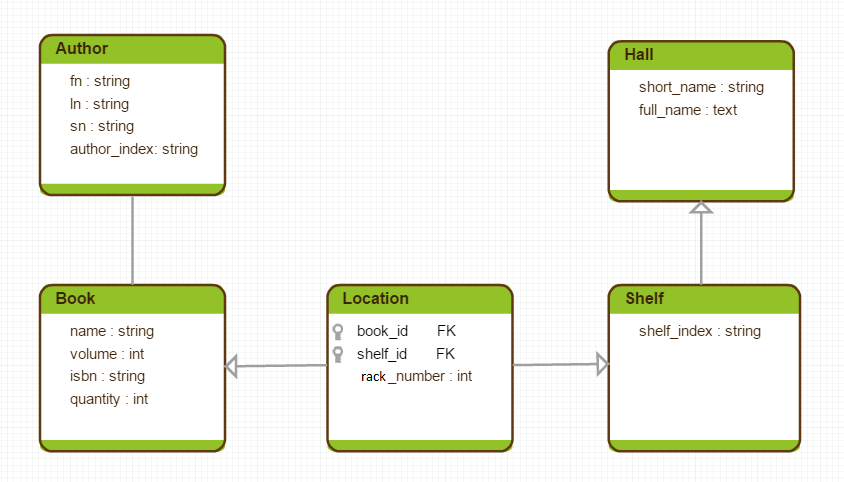
\includegraphics[scale=0.6]{images/erdiagramm.png}
\end{center}
\vspace*{-8mm}
\caption{ER-диаграмма} \label{fig:erdiagramm}
\end{figure}

Что бы сократить действия, которые понадобятся разработчику для интеграции сущностей в веб-приложение, мы будем
использовать scaffolding. По своей сути это утилита командной строки, доступная при работе с Ruby on Rails, которая
генерирует ряд файлов и заполняет их содержимое.

Покажем на примере создания сущности \verb|Книги| образец подобной генерации:
\begin{small}
\begin{verbatim}
rails g scaffold Book name:string volume:integer isbn:string quantity:integer
\end{verbatim}
\end{small}

Благодаря scaffold-у, помимо базового файла с миграцией в приложении сгенерировался REST-контроллер
для данной модели, шаблон views. Уже на данном этапе наше приложение будет уметь просматривать, создавать,
удалять объекты книг. Но это не весь функционал, который должна обеспечивать для данной модели ИС.

После того, как мы создали необходимые сущности перейдем к добовлению ограничений
целлостности и добавления индексов в БД, которые требует концептуальная модель.

Продемострируем пример применения ограничения целлостности на физическом уровне
изменив миграцию создания таблицы стеллажей следующим образом:
\begin{small}
\verbatiminput{programms/authors_migrate.rb}
\end{small}

При необходимости добавить ограничение отсутствующее в Ruby on Rails,
нужно вручную прописать его для
таблицы в соответствующем файле миграции. Добавим такое
ограничение для сущности \verb|Стеллаж|
проверив длину авторского указателя (таким же образом в RoR должны быть добавлены
внешние и первичные ключи которые нельзя было указать при создании миграции).
\begin{small}
\verbatiminput{programms/add_check.rb}
\end{small}

Закончив с описанием ограничений для физического уровня необходимо их
продублировать на уровне классов. Для этого в Rails существует механизм
валидаций.

Встроенные доступные валидации объектного уровня представляют
собой более гибкий инструмент ограничений нежели ограничения
для миграций. Но, как и в случае миграций, всегда можно реализовать
свои ограничений целлостности, если это будет необходмо для приложения.

Перенесем описанные нами ранее ограничения для атрибутов стеллажей в их
объектное представление:
\begin{small}
\verbatiminput{programms/validations.rb}
\end{small}

После написания всех валидаций нам осталось прописать лишь ассоциации
представленные на диаграмме в начале раздела.

Связи между сущностями в Ruby on Rails реализуются элементарно: достаточно просто
укзатель наличие связи необходимой размерности в соответствующих моделях.
Исследовав предметную область и имея некоторый опыт в использовании фреймворка,
не будет лишним добавить связь между \verb|Книгой| и \verb|Стеллажом| напрямую.
Отметим, что исходные транзитивные связи не удаляются, а лишь добавляются новые.

Благодаря наличию связей между объектами нам стал доступен поиск связанных
объектов, а так же их изменения и удаления. Для последующей реализации интерфейсов
редактирования сразу несколько сущностей нашего приложения нам
понадобятся вложенные формы.
Включить их можно при помощи опции accepts nested attributes for.

Привидем пример связей для модели \verb|Стеллаж|:
\begin{small}
\verbatiminput{programms/assotiations.rb}
\end{small}

Мы спроектировали систему сущностей для данной предметной области и
реализовали все необходимые ограничения целлостности и ассоциации.
